\documentclass[14pt]{article}
\usepackage[utf8]{inputenc}
\usepackage{listingsutf8}
%\usepackage[T2A]{fontenc}
\usepackage[english]{babel}
\usepackage{amssymb,amsmath,amsfonts,amsbsy}
%\usepackage{mathtext}
%\usepackage{indentfirst}
\usepackage{tabularx}
\usepackage{booktabs}
\usepackage{graphicx}
\usepackage[center]{caption}
\captionsetup{justification=raggedright,singlelinecheck=false}
\usepackage{subcaption}
\usepackage{cite}
\usepackage{enumerate}
\usepackage{enumitem}
%%\usepackage[braket]{qcircuit}
\usepackage{marvosym}
\usepackage{multicol}
\usepackage{comment}
\usepackage{authblk}
\usepackage{lipsum}
%\usepackage{hyperref}
\graphicspath{{figs/}}
%\DeclareGraphicsExtensions{.pdf,.png,.jpg}
%\bibliographystyle{utf8gost780u}
%\usepackage{apacite}
%\bibliographystyle{apacite}

% Print line number page wisely 
%\usepackage[pagewise]{lineno}
%\linenumbers

%\renewcommand\linenumberfont{\normalfont\bfseries\normal}
%\renewcommand\linenumberfont{\normal}

\title{\textbf{Schizophrenia Detection from MR images}}

%\author[1]{Ilia Golub}
\author[]{Ilia Golub}

%\author[1]{Pratit Kandel}

%\author[1]{Prosperity Oguama}
\author[]{Prosperity Oguama}


%\affil[1]{Gonda Multidisciplinary Brain Research Center, Bar-Ilan University, Ramat Gan, Israel}
\affil[]{Gonda Multidisciplinary Brain Research Center, Bar-Ilan University, Ramat Gan, Israel}
%\affil[4]{Institute of Natural Sciences and Mathematics, Ural Federal University, Ekaterinburg, Russia}
%\affil[5]{Department of Cardiology, Clinical Sciences, Lund University, Lund, Sweden}
%\affil[6]{Arrhythmia Clinic, Skane University Hospital, Lund, Sweden}
%\affil[*]{Correspondence: golub.ilia.ilya@gmail.com}

\setcounter{Maxaffil}{0}
\renewcommand\Affilfont{\itshape\small}
\date{}

\usepackage[onehalfspacing]{setspace}

\usepackage{listings}
\renewcommand{\lstlistingname}{Listing}
\lstset{language=Python,
        numbers=left,
        basicstyle=\small\ttfamily,
        breaklines=true,
        showstringspaces=false,
        stepnumber=1,         
        numbersep=5pt,          
        showspaces=false,       
        showtabs=false,         
        %frame=single,          
        tabsize=4,              
        captionpos=b,           
        breakatwhitespace=false,
        escapeinside={\%*}{*)}, 
        texcl=true
        }

\usepackage[left=2.5cm, right=1cm, top=1cm, bottom=2.5cm]{geometry}

\usepackage[
    colorlinks=true,
    linkcolor=blue,
    filecolor=magenta,      
    urlcolor=cyan,
    pdftitle={CW-2},
    pdfauthor={Golub I},
    bookmarks=true,
    linktoc=all,
	final]{hyperref}

\usepackage[nottoc]{tocbibind}

\makeatletter
\renewcommand{\@biblabel}[1]{#1.}
\makeatother

\sloppy

\righthyphenmin=2

\renewcommand{\theenumi}{\arabic{enumi}.}
\renewcommand{\labelenumi}{\arabic{enumi}.} 
\renewcommand{\theenumii}{\arabic{enumii}.} 
\renewcommand{\labelenumii}{\arabic{enumi}.\arabic{enumii}.}
\renewcommand{\theenumiii}{\arabic{enumiii}.} 
\renewcommand{\labelenumiii}{\arabic{enumi}.\arabic{enumii}.\arabic{enumiii}.} 


\DeclareMathOperator{\rot}{rot}		% Определяем операции rot
\DeclareMathOperator{\diverg}{div}	% div
\DeclareMathOperator{\grad}{grad}	% grad
\DeclareMathOperator{\arth}{Arth}    % arc tanh
\DeclareMathOperator{\Ai}{Ai}
\DeclareMathOperator{\Bi}{Bi}

\setcounter{tocdepth}{1}

\begin{document}

% Title
\maketitle

% Abstract
\section{Abstract}

\textbf{Background}\\
\lipsum[1]
\textbf{Aim}: ...

\textbf{Methods}\\
\lipsum[1]

\textbf{Results}\\
\lipsum[1]

\textbf{Conclusion}\\
\lipsum[1]

\textbf{Keywords: schizophrenia, sMRI, CNN}

% Introduction
\section{Introduction}

Schizophrenia (SZ) is a chronic mental disorder affecting 1 in 300 people worldwide, linked to structural brain abnormalities observable via MRI. Machine learning (ML) and deep learning (DL) have advanced SZ diagnosis, yet variability in preprocessing methods—such as noise removal and intensity normalization—remains a major challenge~\cite{Benli2023, Zhang2022}.

Despite progress in CNN-based SZ detection, studies often lack standardized preprocessing pipelines, impacting model reliability and reproducibility. Benchmark datasets~\cite{Oh2020, Verma2023} report high classification accuracies, but inconsistent preprocessing limits comparability.

This project systematically evaluates preprocessing and augmentation techniques (e.g., smoothing, translation) to establish a robust pipeline for SZ detection from MRI. Standardizing these practices could improve the reproducibility and clinical applicability of ML-based diagnostics.

% Methods
\section{Methods}

\subsection{Dataset and Exploratory Data Analysis}

The raw data were obtained from the \href{http://schizconnect.org}{SchizConnect} database (accessed January 1, 2025), which houses structural and functional MRI data. The database provides filtering options to enable users to select data that meets specific criteria including MRI field strength and clinical diagnosis (e.g. schizophrenia, bipolar disorder).

The data obtained originates from the Center of Biomedical Research Excellence (COBRE) [REF!!!] dataset in NifTI format. It includes data from 62 individuals, 30 with schizophrenia and 32 healthy controls. [CHECK!!!]

The data from SchizConnect was filtered based on MRI field strength and clinical diagnosis. We retrieved only images captured with 3T MRI scans. This was done to ensure uniformity of the data obtained.

Clinical data was made available in form of CSV files. The demographic features of the dataset used in this project are presented in Table~\ref{tab:cobre_clinical_demographic}.
\begin{center}
	\begin{table}
        \centering
        \caption{\label{tab:cobre_clinical_demographic}The subjects were selected to give a balanced representation of age and gender distributions in the dataset, prioritizing age distribution, which has been shown to affect model performance (ref).}
        \begin{tabular*}{500pt}{@{\extracolsep\fill}lcccccc@{\extracolsep\fill}}
            \toprule
            & \multicolumn{3}{c}{COBRE}
            \\\cmidrule{2-4}
            & \textbf{Individuals with SZ (n=30)} & \textbf{Healthy controls (n=32)} & \textbf{Total (62)} \\
            \midrule
            Minimum age             & 19  & 18  & 18 \\
            Maximum age 		    & 66  & 65 & 66  \\
            Average age             & 39.6 & 41 & 40.3	\\
            Gender (Male/ Female)   & 19/11 & 17/15 & 36/26	\\
            \bottomrule
        \end{tabular*}
    \end{table}    
\end{center}

%
\subsection{Image Preprocessing}

% General thoughts
The major idea behind preprocessing was to establish a standardized pipeline that ensures consistency in the quality and content of the MRI data. This pipeline addressed common issues such as noise, intensity variations, and artifacts, which can affect the performance of machine learning models.

We experimented with different combinations of preprocessing and data augmentation techniques to determine which pipeline yields the best performance of the ML/DL models regarding recall rate, precision, and F1 score.

In order to find the best combination of hyperparameters for each preprocessing method, we performed a grid search and measured the quality metrics of the processed image using a custom test function.

Table~\ref{tab:preprocessing_pipeline} presents the preprocessing techniques used and their respective hyperparameters and tools used. Figure~\ref{fig:test_pipeline} gives a visual representation of the conducted tests.
%
\begin{figure}[h]
    \centering
    
\includegraphics[width=0.4\textwidth]{./figs/empty.pdf} % test_pipeline.png
    \caption{Tests pipeline for MRI data.}\label{fig:test_pipeline}
\end{figure}

\subsubsection{Resampling}

The first step of the pipeline is resampling the image to a standard resolution to ensure uniform input for the model and consistent noise and signal profiles.

\subsubsection{intensity normalization}

The second step of the pipeline is normalization of voxel intensities to a consistent range to maintain the relative scale of the data and produce values in a fixed range to satisfy models expectations. The adopted method scales the data to a range of [0, 1].

Normalization also improves the results of brain extraction by helping the algorithm better distinguish between brain and non-brain regions.

Intensity distributions were inspected to ensure normalization has not distorted the data.

\subsubsection{Brain extraction}

The third step of the pipeline is a brain extraction. The purpose of this stage is to
\begin{itemize}
    \item remove non-brain regions in order to minimizes noise, making it easier for the network to focus on relevant features;
    \item subsequently enhance the network's performance, especially in a schizophrenia detection task where small differences in brain anatomy are crucial;
    \item ensure that the input images are more consistent in terms of content, which can help the model generalize better.
\end{itemize}

The generated brain mask was refined by closing gaps and removing small regions. The mask was also used as a leverage for the cropping step.

\subsubsection{Cropping}

The fourth step of the pipeline is cropping the brain region to a consistent size across scans.

\subsubsection{Smoothing}

The fifth step of the pipeline is smoothing the brain region to reduce noise and variability introduced by acquisition artifacts, enhancing the overall quality of the images. This was done to ensure that the downstream tasks are more robust and the model training is more effective. We used a Gaussian filter to reduce high-frequency noise while preserving edges to some extent. Since the neural network performed a classification task, moderate smoothing was carried out to focus on broader patterns.

The sixth step of the pipeline is normalization of the smoothed image to ensure that ...

\subsubsection{Validation}

The impact of preprocessing on the data's integrity and quality was assessed using a combination of a visual inspection and quantitative metrics. The visual inspection involved plotting a few slices of the MRI before and after each preprocessing step. Validation was performed to ensure that preprocessing steps did not introduce artifacts or distort anatomical structures, and to ensure consistency of the processed images.

Quantitative metrics included Signal-to-Noise Ratio (SNR), Contrast-to-Noise Ratio (CNR), Peak Signal-to-Noise Ratio (PSNR), and 
Structural Similarity Index (SSIM). 

Relative PSNR for one image. Using a hypothetical "ideal" signal (the maximum intensity value as a baseline), a relative PSNR for one image was calculated. This relative PSNR was used as a way to assess the "quality" of a single image compared to a theoretical perfect image of uniform intensity.

A binary mask was computed using Otsu's thresholding to explicitly select a background region for noise estimation.

The metrics were computed for the entire 3D volume to assess the overall quality or similarity of the entire MRI dataset, capturing global differences.
\begin{center}
    \begin{table}
        \centering
        \caption{\label{tab:preprocessing_pipeline}Preprocessing techniques used in the study.}
        \begin{tabular*}{500pt}{@{\extracolsep\fill}lcc@{\extracolsep\fill}}
            \toprule
            \textbf{Preprocessing Step} & \textbf{Hyperparameters} & \textbf{Tools} \\
            \midrule
            Resampling & Voxel size: \texttt{2x2x2} & Nibabel library \\
            Intensity Normalization & Min-max scaling: [0, 1] & NumPy \\
            Brain Extraction & Modality: T1, U-net & ANTsPyNet \\
            Cropping & Size: based on the largest bounding box among all images & scikit-image, NumPy \\
            Smoothing & Gaussian filter: sigma=0.5 & SciPy \\
            \bottomrule
            \end{tabular*}
    \end{table}
\end{center}
%
\subsection{Data Augmentation}

According to typical variations in brain MRI scans, the following transformations with corresponding parameters were applied to the images:
\begin{itemize}
    %\item[\textbf{Option 1}]  \textbf{Shearing.} A shearing angle is selected randomly within the range $\left[-15^{\circ}, 15^{\circ}\right]$ and A shearing operation is applied within the x and y-axis. This operation is repeated 10 times with 10 different shearing angles. By this method, 10 images are generated from an original image;
    \item[\textbf{Option 1}] \textbf{Translation}. The operation is applied on the x and y-axis and repeated 10 times by using different values sampled randomly within the range $\left[-10, 10\right]$. By this method, 10 images are generated from an original image.
    \item[\textbf{Option 2}] \textbf{Rotation.} Rotation angles are selected randomly within the range  $\left[-10^{\circ}, 10^{\circ}\right]$ and clockwise rotations are applied using 10 different angle values. 10 images are generated from an original image by this method.
    \item[\textbf{Option 3}] \textbf{Gaussian noise addition.} Noise addition is applied by \mbox{$I=I+R*I*std+mean$}, where $I$ refers to the image, $R$ refers to the Noise. The noise to be added is generated using a Gaussian distribution. The variance of the distribution is computed from the input images while the mean value is set to zero. In this study, three different fixed values (0.1, 0.2, and 0.3) are used and 3 images are generated from an input image.
    %\item[\textbf{Option 4}] \textbf{Gaussian noise addition followed by rotation.} 30 images are generated from an input image by this method.
    %\item[\textbf{Option 5}] \textbf{Clockwise rotation followed by translation.} Rotation angles are selected randomly within the range $\left[-25^{\circ}, 25^{\circ}\right]$ and translation is applied on the x and y-axis by using different values sampled randomly within the range $\left[-15^{\circ}, 15^{\circ}\right]$. This successive operation is applied 10 times, and 10 images are generated from an input image by this method.
    %\item[\textbf{Option 6}] \textbf{Translation followed by shearing.} The translation step is applied on the x and y-axis with different values sampled randomly within the range $\left[-15, 15\right]$. In the shearing step, an angle is selected randomly within the range $\left[-15^{\circ}, 15^{\circ}\right]$, and shearing is applied within the x and y-axis. The subsequent operations are applied 10 times, and 10 images are generated from an input image by this method.
    %\item[\textbf{Option 7}] \textbf{Translation, shearing, and rotation.} Operations are applied subsequently. Implementation of the translation and shearing operations are performed as explained in the previous method. In the rotation step, a random angle is selected within the range $\left[-25^{\circ}, 25^{\circ}\right]$ clockwise rotation is applied. The successive operations are applied 10 times, and 10 images are generated from an input image by this method.
\end{itemize}

The augmented samples were plotted to ensure the transformations don't distort anatomical features.

%
\subsection{Model architectures}

Convolutional Neural Networks (CNNs) are commonly used in the literature for this task [REFS!!]. However, a few papers explored the use of support vector machines for image classification [REFS!!]. To gain a full understanding of both approaches, we decided on the combination of a pretrained deep neural network for feature extraction and a support vector classifier for binary classification. The ReNet-18 architecture was selected for its balance between computational load and accuracy. Cross validation was performed with the support vector classifier (SVC) to choose the best hyperparameters, and the hyperparameters that yielded the best results were the radial basis function (RBF) kernel, a gamma value of 0.0001 and a C parameter value of 100. Each 2D slice of the images were fed into the ResNet-18 model as NumPy arrays of dimension $224x224$. This input size corresponds to the size of the images in the ImageNet dataset that was used to train ResNet-18 and was selected for compatibility with the pretrained weights of the ResNet-18 model. Figure~\ref{fig:training_architecture} gives a representation of the training architecture and flow.
%
\begin{figure}
    \centering
    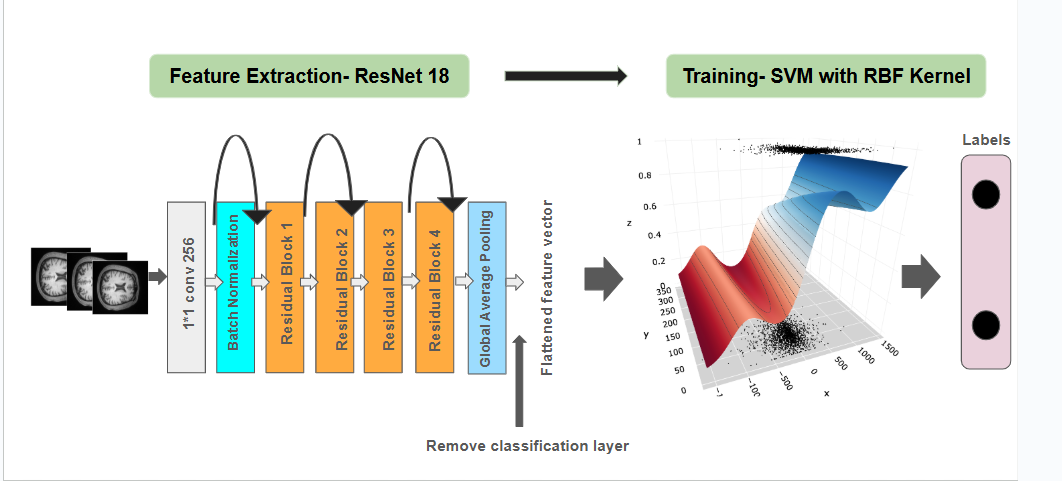
\includegraphics[width=0.4\textwidth]{./figs/model_architecture.png} % training_architecture.png
    \caption{Training architecture and flow.}\label{fig:training_architecture}
\end{figure}

%
\subsection{Training and validation}

The dataset was split into a training set (80\%) and a validation set (20\%). 

Accuracy, recall, precision, and F1-score were calculated to asses the performance of the SVC.

% Results
\section{Results}

\subsection{Image Preprocessing}

The results presented in Table~\ref{tab:model_metrics_preprocessing} demonstrate the impact of various preprocessing methods on classification performance. The baseline model using raw images (0) achieved an accuracy of 0.51, with an F1-score of 0.63. Applying resampling (1) alone did not alter these results, suggesting that resampling alone does not introduce substantial benefits.

Normalization (2) improved accuracy to 0.56 and F1-score to 0.67, indicating that standardizing intensity values enhances model performance. Brain extraction (3) yielded a slightly lower accuracy (0.54) but a notable increase in recall (0.78), which suggests that removing non-brain tissues helps capture more positive instances but may introduce a trade-off in precision.

Cropping (4) led to the highest accuracy (0.57) and an F1-score of 0.69, highlighting its effectiveness in improving signal-to-noise ratio. Smoothing (5) showed a moderate impact, improving results compared to the raw data but not outperforming other methods.

When combining preprocessing techniques, the pattern is less straightforward. The combination of resampling, normalization, and brain extraction (1+2+3) resulted in the highest recall (0.80) while maintaining a strong F1-score (0.69). However, adding cropping (1+2+3+4) caused a drastic performance drop, with accuracy declining to 0.44 and F1-score to 0.54. The full pipeline (1+2+3+4+5) slightly improved over this but still underperformed compared to individual preprocessing steps.
\begin{center}
	\begin{table}[t]
		\centering
		\caption{\label{tab:model_metrics_preprocessing}Desct}
		\begin{tabular*}{500pt}{@{\extracolsep\fill}lcccc@{\extracolsep\fill}}
			\toprule
		     \textbf{Preprocessing method} &\textbf{Accuracy} &  \textbf{Recall} &\textbf{Precision} &\textbf{F1-score}\\
			\midrule
			Raw (0) & 0.51 & 0.67 & 0.60 & 0.63 \\
			Resampling (1) & 0.51 & 0.67 & 0.60 & 0.63 \\
			Normalization (2) & 0.56 & 0.69 & 0.64 & 0.67 \\
			Brain extraction (3) & 0.54 & 0.78 & 0.60 & 0.68 \\
			Cropping (4) & 0.57 & 0.76 & 0.63 & 0.69 \\
			Smoothing (5) & 0.55 & 0.71 & 0.62 & 0.66 \\
            1+2 & 0.56 & 0.76 & 0.57 & 0.65 \\
            1+2+3 & 0.55 & 0.80 & 0.61 & 0.69 \\
            1+2+3+4 & 0.44 & 0.53 & 0.56 & 0.54 \\
            1+2+3+4+5 & 0.48 & 0.60 & 0.58 & 0.59 \\
			\bottomrule
		\end{tabular*}
	\end{table}
\end{center}

\subsection{Data Augmentation}

According to the results, Table~\ref{tab:model_meetrics_augmentation}
\begin{center}
	\begin{table}[t]
		\centering
		\caption{\label{tab:model_meetrics_augmentation}Desct}
		\begin{tabular*}{500pt}{@{\extracolsep\fill}lcccc@{\extracolsep\fill}}
			\toprule
			\textbf{Augmentation method} &\textbf{Accuracy} &  \textbf{Recall} &\textbf{Precision} &\textbf{F1-score}\\
			\midrule
			Raw (0) & 0.51 & 0.67 & 0.60 & 0.63 \\
			Translation (1) & 0.75 & 0.84 & 0.74 & 0.79 \\
			Rotation (2) & 0.79 & 0.81 & 0.78 & 0.80 \\
			Gaussian Noise (3) & 0. & 0. & 0. & 0. \\
			\bottomrule
		\end{tabular*}
	\end{table}
\end{center}

% Discussion
\section{Discussion}

This study investigated...

These results suggest that while certain preprocessing steps (e.g., normalization, brain extraction, and cropping) contribute positively when applied individually, combining them does not necessarily yield additive benefits. Over-processing may introduce distortions that hinder model generalization.

The methods used for brain MR image augmentation have some limitations or drawbacks. For instance, in a study (Isensee et al. 2020), the augmentation approach uses elastic deformations, which add shape variations. However, the deformations can bring lots of damage and noise when the deformation field is varied seriously. Also, the generated images seem not to be realistic and natural. It has been shown in the literature that widely used elastic deformations produce unrealistic brain MR images (Mok and Chung 2018).

augmentation with the combination of shearing and salt-and-pepper noise addition is the least efficient approach for augmentation in improving classification performance 

% Discuss When Brain Extraction May Not Be Necessary

% Discuss Metrics for Each 2D Slice (Slice-wise Approach):


% Conclusion
\section{Conclusion}

% Random text
\lipsum[9-10]



% Formalities
\section*{Acknowledgements}

...

\subsection*{Author contributions}

\textbf{Conception}: Prosperity Oguama, Ilia Golub; \textbf{Data Acquisition}: Ilia Golub; \textbf{Preprocessing Pipeline Development}: ...; \textbf{Preprocessing Pipeline Testing}: ...; \textbf{Data Augmentation Pipeline Testing}: ...; \textbf{Neural Network Building}: ...; \textbf{Neural Network Testing}: ...; \textbf{Drafting \& Editing}: Ilia Golub, Prosperity Oguama. All authors contributed to the study, read, revised and approved the final manuscript.

\subsection*{Data availability statement}
The data underlying this article is publicly available and accessible through \hyperlink{Schizconnect}{http://schizconnect.org/}.

\subsection*{Financial disclosure}

The authors report no financial disclosure.

\subsection*{Conflict of interest}

The authors declare no potential conflict of interests.

\renewcommand{\baselinestretch}{1.5} % Полуторный межстрочный интервал
%\singlespacing
%\renewcommand\bibname{Bibliography}
\bibliographystyle{abbrv} %abbrv
\phantomsection     % для корректных ссылок на
\cleardoublepage    % библиографию
\bibliography{paper}


\end{document}